% FriendlyFace — ICDF2C 2026 Submission
% Compile with: pdflatex paper.tex && bibtex paper && pdflatex paper.tex && pdflatex paper.tex
\documentclass[conference]{IEEEtran}

\usepackage{amsmath,amssymb,amsfonts}
\usepackage{algorithmic}
\usepackage{graphicx}
\graphicspath{{figures/}}
\usepackage{textcomp}
\usepackage{xcolor}
\usepackage{hyperref}
\usepackage{booktabs}
\usepackage{multirow}
\usepackage{url}
\usepackage{listings}
\usepackage{enumitem}

\lstset{
  basicstyle=\ttfamily\small,
  breaklines=true,
  frame=single,
  language=Python,
  keywordstyle=\color{blue},
  commentstyle=\color{gray},
}

\hypersetup{
  colorlinks=true,
  linkcolor=black,
  citecolor=black,
  urlcolor=blue,
}

\begin{document}

\title{FriendlyFace: A Complete Implementation of Forensic-Friendly AI for Facial Recognition with Blockchain Provenance, Federated Fairness, and Regulatory Compliance}

\author{
\IEEEauthorblockN{Dico Angelo}
\IEEEauthorblockA{Metaventions AI\\
\url{friendlyface.metaventionsai.com}\\
\url{github.com/Dicoangelo/FriendlyFace}}
}

\maketitle

\begin{abstract}
Facial recognition systems are increasingly deployed in law enforcement, border security, and access control, yet no existing commercial or academic system provides end-to-end forensic accountability. Mohammed's ICDF2C 2024 schema proposes a six-layer forensic-friendly architecture for AI facial recognition---spanning recognition, federated learning, blockchain forensic integrity, fairness auditing, explainability, and consent governance---but provides no implementation. We present FriendlyFace, the first complete implementation of this schema, integrating five additional state-of-the-art research contributions: zero-knowledge biometric verification via Schnorr proofs (BioZero), trustworthy blockchain-based federated learning with Ed25519 DID:key credentials (TBFL), fairness-aware federated learning with differential privacy (FedFDP), saliency-driven decomposition for explainability (SDD), and automated EU AI Act compliance reporting. FriendlyFace comprises 15,000 lines of Python backend code, 7,700 lines of React frontend code, 1,545 tests achieving 93\% coverage, 20 database tables, and 84+ REST API endpoints. Every operation produces a \texttt{ForensicEvent} that is SHA-256 hash-chained, inserted into an append-only Merkle tree, and linked into a directed acyclic provenance graph---forming self-verifiable forensic bundles suitable for court presentation. We introduce the ForensicSeal, a composite cryptographic attestation combining W3C Verifiable Credentials, Schnorr ZK proofs, and six-layer compliance checking, with measured issuance latency of 3.3\,ms and verification latency of 6.0\,ms. FriendlyFace is deployed at \url{friendlyface.metaventionsai.com} and open-sourced at \url{github.com/Dicoangelo/FriendlyFace}.
\end{abstract}

\begin{IEEEkeywords}
forensic AI, facial recognition, blockchain provenance, federated learning, differential privacy, explainability, bias auditing, verifiable credentials, zero-knowledge proofs, EU AI Act
\end{IEEEkeywords}

%===================================================================
\section{Introduction}
%===================================================================

Facial recognition technology has achieved remarkable accuracy in controlled settings, with commercial systems from NEC, Cognitec, and others reporting verification rates exceeding 99\% on benchmark datasets~\cite{grother2019frvt}. These systems are now deployed across law enforcement agencies, border control checkpoints, and commercial access control systems worldwide. However, this widespread deployment has occurred without corresponding advances in forensic accountability---the ability to independently verify, audit, and challenge the decisions made by these systems.

The absence of forensic accountability creates three critical problems. First, \textbf{evidentiary integrity}: when a facial recognition match is used as evidence in criminal proceedings, there is no standardized mechanism to verify that the recognition pipeline was not tampered with, that the training data was unbiased, or that the specific inference was explainable. Second, \textbf{regulatory compliance}: the EU AI Act (Regulation 2024/1689) classifies biometric identification systems as ``high-risk'' and mandates transparency, human oversight, and bias monitoring---requirements that no current production system satisfies end-to-end. Third, \textbf{public trust}: high-profile failures in facial recognition accuracy across demographic groups~\cite{buolamwini2018gender} have eroded confidence in these systems.

Mohammed's ICDF2C 2024 schema~\cite{mohammed2024forensic} addresses this gap at the architectural level by proposing a six-layer forensic-friendly framework: (1)~Recognition Engine, (2)~Federated Learning, (3)~Blockchain Forensic Layer, (4)~Fairness Auditor, (5)~Explainability, and (6)~Consent and Governance. However, the schema remains theoretical: no reference implementation exists, no integration strategy is provided, and no quantitative evaluation demonstrates feasibility.

\textbf{Contributions.} We present FriendlyFace, the first complete implementation of Mohammed's six-layer schema, with the following contributions:

\begin{enumerate}[leftmargin=*]
\item \textbf{Full-stack implementation} of all six layers with a unified forensic backbone: every operation produces a hash-chained \texttt{ForensicEvent} linked into a Merkle tree and provenance DAG.

\item \textbf{Integration of five additional SOTA research papers}: BioZero~\cite{biozero2024}, TBFL~\cite{tbfl2026}, FedFDP~\cite{feddp2024}, SDD~\cite{sdd2025}, and EU AI Act compliance~\cite{euaiact2025}.

\item \textbf{ForensicSeal}: a composite cryptographic attestation combining W3C Verifiable Credentials, Schnorr ZK proofs, and six-layer compliance checking into a single, publicly verifiable seal---with measured issuance latency of 3.3\,ms and verification latency of 6.0\,ms.

\item \textbf{Quantitative evaluation} across integrity verification, fairness auditing, explainability coverage, privacy accounting, and regulatory compliance.

\item \textbf{Open-source reference implementation} with 1,545 tests (93\% coverage) and a production deployment.
\end{enumerate}

%===================================================================
\section{Related Work}
%===================================================================

\subsection{Commercial Facial Recognition Systems}

Commercial systems have achieved high accuracy but lack forensic accountability. \textbf{Clearview AI} provides large-scale face search but no bias auditing, explainability, or cryptographic integrity~\cite{hill2020clearview}. \textbf{NEC NeoFace} achieves top-tier FRVT accuracy but lacks federated learning, consent management, and self-verifiable evidence packages~\cite{nec2023}. \textbf{Amazon Rekognition} was withdrawn from law enforcement use in 2020 due to bias concerns~\cite{aws2023}. \textbf{Cognitec FaceVACS} provides SDK-level recognition with liveness detection but lacks fairness auditing and consent governance~\cite{cognitec2023}.

\subsection{Academic Prototypes}

Several prototypes address individual layers. \textbf{FairFace}~\cite{karkkainen2021fairface} demonstrates bias-aware training without forensic logging. \textbf{Grad-CAM}~\cite{selvaraju2017gradcam} and \textbf{LIME}~\cite{ribeiro2016lime} provide post-hoc explainability without forensic chain integration. Blockchain identity systems~\cite{muhle2018ssi} demonstrate tamper-evident records without recognition integration. \textbf{FATE}~\cite{liu2021fate} and \textbf{PySyft}~\cite{ryffel2018pysyft} provide privacy-preserving FL without forensic logging or bias auditing.

\subsection{Forensic AI Frameworks}

Mohammed's ICDF2C 2024 schema~\cite{mohammed2024forensic} is the most comprehensive proposed architecture. Other proposals include blockchain audit trails for ML~\cite{sarpatwar2020auditable} and DP frameworks for biometrics~\cite{feddp2024}, but none integrate all six dimensions into a single operational system.

\subsection{Comparative Analysis}

Table~\ref{tab:comparison} compares FriendlyFace against commercial and academic systems across eleven forensic accountability features.

\begin{table*}[t]
\centering
\caption{Feature comparison across forensic accountability dimensions. $\bullet$ = implemented; $\circ$ = partial; -- = not implemented.}
\label{tab:comparison}
\begin{tabular}{lccccccc}
\toprule
\textbf{Feature} & \textbf{Clearview} & \textbf{NEC} & \textbf{Rekognition} & \textbf{Cognitec} & \textbf{FairFace} & \textbf{Grad-CAM} & \textbf{FriendlyFace} \\
\midrule
Hash-chained event log & -- & -- & -- & -- & -- & -- & $\bullet$ \\
Merkle tree verification & -- & -- & -- & -- & -- & -- & $\bullet$ \\
Provenance DAG & -- & -- & -- & -- & -- & -- & $\bullet$ \\
Self-verifiable bundles & -- & -- & -- & -- & -- & -- & $\bullet$ \\
Federated learning & -- & -- & -- & -- & -- & -- & $\bullet$ \\
Bias auditing & -- & -- & $\circ$ & -- & $\bullet$ & -- & $\bullet$ \\
Explainability (LIME/SHAP/SDD) & -- & -- & -- & -- & -- & $\circ$ & $\bullet$ \\
Consent management & -- & -- & -- & -- & -- & -- & $\bullet$ \\
ZK proof verification & -- & -- & -- & -- & -- & -- & $\bullet$ \\
EU AI Act compliance & -- & -- & -- & -- & -- & -- & $\bullet$ \\
ForensicSeal (composite VC) & -- & -- & -- & -- & -- & -- & $\bullet$ \\
\bottomrule
\end{tabular}
\end{table*}

%===================================================================
\section{System Architecture}
%===================================================================

\subsection{Overview}

FriendlyFace implements Mohammed's six-layer schema as a monolithic Python application with a React frontend, organized around a central forensic backbone. Figure~\ref{fig:architecture} illustrates the high-level architecture.

\begin{figure}[h]
\centering
\includegraphics[width=\columnwidth]{fig1-architecture.png}
\caption{FriendlyFace six-layer architecture with ForensicSeal. Layer~3 (Blockchain Forensic Layer) serves as the central backbone receiving forensic events from all other layers.}
\label{fig:architecture}
\end{figure}

\subsection{Forensic Backbone (Layer 3)}

The forensic backbone unifies all six layers through four interconnected structures:

\textbf{Hash-Chained Event Log.} Every operation produces a \texttt{ForensicEvent}. Each event's hash is computed as:
\begin{equation}
H_i = \text{SHA-256}(\text{canonical}(e_i) \| H_{i-1})
\end{equation}
where $\text{canonical}(e_i)$ is the deterministic JSON serialization of event $e_i$'s hashable fields, and $H_{i-1}$ is the hash of the preceding event. The genesis event uses sentinel $H_0 = \text{``GENESIS''}$.

\textbf{Append-Only Merkle Tree.} Event hashes are inserted as leaves following the BioZero pattern~\cite{biozero2024}. The tree supports $O(\log n)$ inclusion proofs. The Merkle root serves as a compact commitment to the entire event history.

\textbf{Provenance DAG.} A directed acyclic graph tracks data lineage:
\begin{equation}
\text{dataset} \to \text{training} \to \text{model} \to \text{inference} \to \text{explanation} \to \text{bundle}
\end{equation}
Relations follow the W3C PROV ontology~\cite{moreau2013prov}: \texttt{DERIVED\_FROM}, \texttt{GENERATED\_BY}, \texttt{USED}, and \texttt{ATTRIBUTED\_TO}.

\textbf{Forensic Bundles.} A \texttt{ForensicBundle} aggregates related events across all six layers. Each bundle contains ordered event IDs, Merkle proofs, provenance chain, layer artifacts, a Schnorr ZK proof, an Ed25519 DID-signed Verifiable Credential, and a composite bundle hash:
\begin{equation}
H_{\text{bundle}} = \text{SHA-256}(\text{canonical}(\text{id}, \text{created\_at}, \text{event\_ids}, \ldots))
\end{equation}

\begin{figure}[h]
\centering
\includegraphics[width=\columnwidth]{fig3-data-structures.png}
\caption{Forensic data structures: SHA-256 hash chain for tamper detection, Merkle tree for efficient inclusion proofs, and provenance DAG for lineage tracking, aggregated into self-verifiable forensic bundles.}
\label{fig:data-structures}
\end{figure}

\subsection{Layer 1: Recognition Engine}

The recognition engine implements multi-modal biometric recognition. \textbf{Face Recognition} uses PCA dimensionality reduction followed by SVM classification on aligned 112$\times$112 grayscale images. \textbf{Voice Recognition} uses MFCC feature extraction with cosine similarity. \textbf{Multi-Modal Fusion} combines scores:
\begin{equation}
s_{\text{fused}}(i) = w_f \cdot s_{\text{face}}(i) + w_v \cdot s_{\text{voice}}(i)
\end{equation}
where $w_f + w_v = 1$ (default $w_f = 0.6$, $w_v = 0.4$).

\subsection{Layer 2: Federated Learning}

\textbf{FedAvg} aggregates client updates with forensic logging. \textbf{DP-FedAvg}~\cite{feddp2024} adds per-client gradient clipping:
\begin{equation}
\tilde{\Delta}_c = \Delta_c \cdot \min\left(1, \frac{C}{\|\Delta_c\|_2}\right)
\end{equation}
and calibrated Gaussian noise with $\sigma = \sqrt{2 \ln(1.25/\delta)} / (\epsilon \cdot n)$.

\textbf{Poisoning Detection} flags malicious updates when $\|\Delta_c\|_2 > \tau \cdot \text{median}(\|\Delta_1\|_2, \ldots, \|\Delta_n\|_2)$ with $\tau = 3.0$.

\subsection{Layer 4: Fairness Auditor}

Two group fairness metrics are computed:

\textbf{Demographic Parity Gap:}
\begin{equation}
\text{DP}_{\text{gap}} = \max_g \text{PPR}(g) - \min_g \text{PPR}(g)
\end{equation}

\textbf{Equalized Odds Gap:}
\begin{equation}
\text{EO}_{\text{gap}} = \max\!\left(\max_g \text{TPR}(g) - \min_g \text{TPR}(g),\; \max_g \text{FPR}(g) - \min_g \text{FPR}(g)\right)
\end{equation}

Threshold breaches trigger \texttt{SECURITY\_ALERT} events.

\subsection{Layer 5: Explainability}

Three complementary methods are provided: \textbf{LIME}~\cite{ribeiro2016lime} (grid-based superpixel segmentation), \textbf{KernelSHAP}~\cite{lundberg2017shap} (Shapley value approximation), and \textbf{SDD Saliency}~\cite{sdd2025} (finite-difference gradient decomposition into seven facial regions):
\begin{equation}
g_i = \frac{f(x + \epsilon \cdot e_i) - f(x - \epsilon \cdot e_i)}{2\epsilon}
\end{equation}

All methods produce \texttt{ForensicEvent(EXPLANATION\_GENERATED)} records with provenance links.

\subsection{Layer 6: Consent and Governance}

\textbf{Consent Management} uses an append-only engine with \texttt{require\_consent()} gating. \textbf{Cryptographic Erasure} (GDPR Art.\ 17) uses per-subject AES-256-GCM keys. \textbf{EU AI Act Compliance} reports cover Articles 5 and 14:
\begin{equation}
S_{\text{compliance}} = 0.30 C_{\text{consent}} + 0.25 C_{\text{bias}} + 0.25 C_{\text{explain}} + 0.20 C_{\text{bundle}}
\end{equation}

%===================================================================
\section{Implementation}
%===================================================================

\subsection{Technology Stack}

FriendlyFace uses FastAPI (async REST), Pydantic (type safety), SQLite/Supabase (storage), scikit-learn (PCA+SVM), PyNaCl (Ed25519), and React~19 (frontend). Core forensic logic uses only Python stdlib and hashlib. Table~\ref{tab:scale} summarizes implementation scale.

\begin{table}[h]
\centering
\caption{Implementation metrics.}
\label{tab:scale}
\begin{tabular}{lr}
\toprule
\textbf{Metric} & \textbf{Value} \\
\midrule
Backend Python LOC & 14,974 \\
Test Python LOC & 20,039 \\
Frontend TypeScript/React LOC & 7,692 \\
Total LOC & 42,705 \\
Test functions & 1,545 \\
Test coverage & 93\% \\
Database tables & 20 \\
API endpoints & 84+ \\
Authentication providers & 3 \\
\bottomrule
\end{tabular}
\end{table}

\subsection{Hash-Chained Forensic Events}

The \texttt{ForensicEvent} model contains seven hashable fields: \texttt{id}, \texttt{event\_type} (one of 13 types), \texttt{timestamp}, \texttt{actor}, \texttt{payload}, \texttt{previous\_hash}, and \texttt{sequence\_number}. The system defines 13 event types spanning all six layers.

\subsection{Merkle Tree Verification}

The append-only Merkle tree supports: append ($O(1)$ amortized), root computation ($O(n)$), inclusion proof generation ($O(\log n)$), and proof verification ($O(\log n)$). Verification recomputes the root from the leaf using the proof path.

\subsection{Provenance DAG}

Each \texttt{ProvenanceNode} contains entity type, entity ID, parent node UUIDs, relation types, and an integrity hash. The DAG supports chain retrieval, children enumeration, and per-chain integrity verification.

\subsection{Forensic Bundles}

Bundle creation orchestrates all six layers: event collection, artifact gathering, Merkle proof generation, Schnorr ZK proof, DID-signed VC issuance, and composite hash sealing. Verification checks seven dimensions: bundle hash integrity, Merkle proofs, provenance chain, layer artifacts, ZK proof, DID credential, and overall status.

\subsection{Zero-Knowledge Proofs (Schnorr)}

Following BioZero~\cite{biozero2024}, a non-interactive Schnorr identification protocol via the Fiat-Shamir heuristic is used. Secret $x = \text{SHA-256}(\text{bundle\_hash}) \bmod q$, commitment $r = g^k \bmod p$, challenge $c = \text{SHA-256}(g \| r \| y) \bmod q$, response $s = (k - c \cdot x) \bmod q$. Verification: $g^s \cdot y^c \equiv r \pmod{p}$.

\subsection{DID:key and Verifiable Credentials}

Following TBFL~\cite{tbfl2026}, Ed25519 keypairs are encoded using the \texttt{did:key} method with multicodec prefix \texttt{0xed01}. W3C Verifiable Credentials with \texttt{Ed25519Signature2020} proof type are issued for each bundle.

\subsection{ForensicSeal}

The ForensicSeal is a composite cryptographic attestation that binds all six layers of a forensic bundle into a single, publicly verifiable credential.

\textbf{W3C Verifiable Credential Format.} Each seal is a W3C VC v1.0 document with type \texttt{["VerifiableCredential", "ForensicSeal"]}. The credential subject contains the bundle ID, composite hash, layer coverage bitmap, compliance score, and expiry timestamp.

\textbf{Six-Layer Compliance Checking.} Before seal issuance, a six-layer compliance check validates:
\begin{enumerate}[leftmargin=*]
\item \textit{Consent}: active, non-expired consent for all subjects.
\item \textit{Recognition}: hash-chained integrity and provenance links.
\item \textit{Fairness}: bias audit existence with metrics within threshold.
\item \textit{Explainability}: at least one explanation method applied.
\item \textit{Forensic integrity}: Merkle proofs, hash chain, ZK proof, DAG.
\item \textit{Governance}: compliance score $\geq 70$.
\end{enumerate}

\textbf{ZK Proof for Evidence.} The ForensicSeal includes a Schnorr ZK proof demonstrating knowledge of the bundle hash without revealing content---enabling cross-jurisdictional verification without full evidence disclosure.

\textbf{Public Verification.} ForensicSeals are verified without authentication via \texttt{POST /verify/\{bundle\_id\}}. Measured verification latency: 6.0\,ms.

\textbf{Continuous Compliance.} Seals carry expiry timestamps (default 90 days, configurable 7--365). Renewal triggers fresh six-layer compliance checks and links to the previous seal via \texttt{previous\_seal\_id}, creating a verifiable compliance chain. Revocation is irreversible and cryptographically recorded in the hash chain. Seal issuance completes in 3.3\,ms.

\begin{figure}[h]
\centering
\includegraphics[width=\columnwidth]{fig2-seal-lifecycle.png}
\caption{ForensicSeal lifecycle: issuance with 6-layer compliance checks (threshold $\geq 80\%$), public verification without authentication, continuous compliance via expiry and renewal, and irreversible revocation.}
\label{fig:seal-lifecycle}
\end{figure}

\textbf{Compliance Proxy.} FriendlyFace includes a compliance proxy (\texttt{POST /proxy/recognize}) that transparently wraps third-party recognition APIs (NEC NeoFace, Amazon Rekognition, Cognitec FaceVACS) with forensic logging. Before forwarding, the proxy checks consent and logs an \texttt{inference\_request} event. After receiving the upstream response, it logs an \texttt{inference\_result} event with the response hash and latency. Accumulated proxy events feed into bias audits and ForensicSeal compliance scoring.

\begin{figure}[h]
\centering
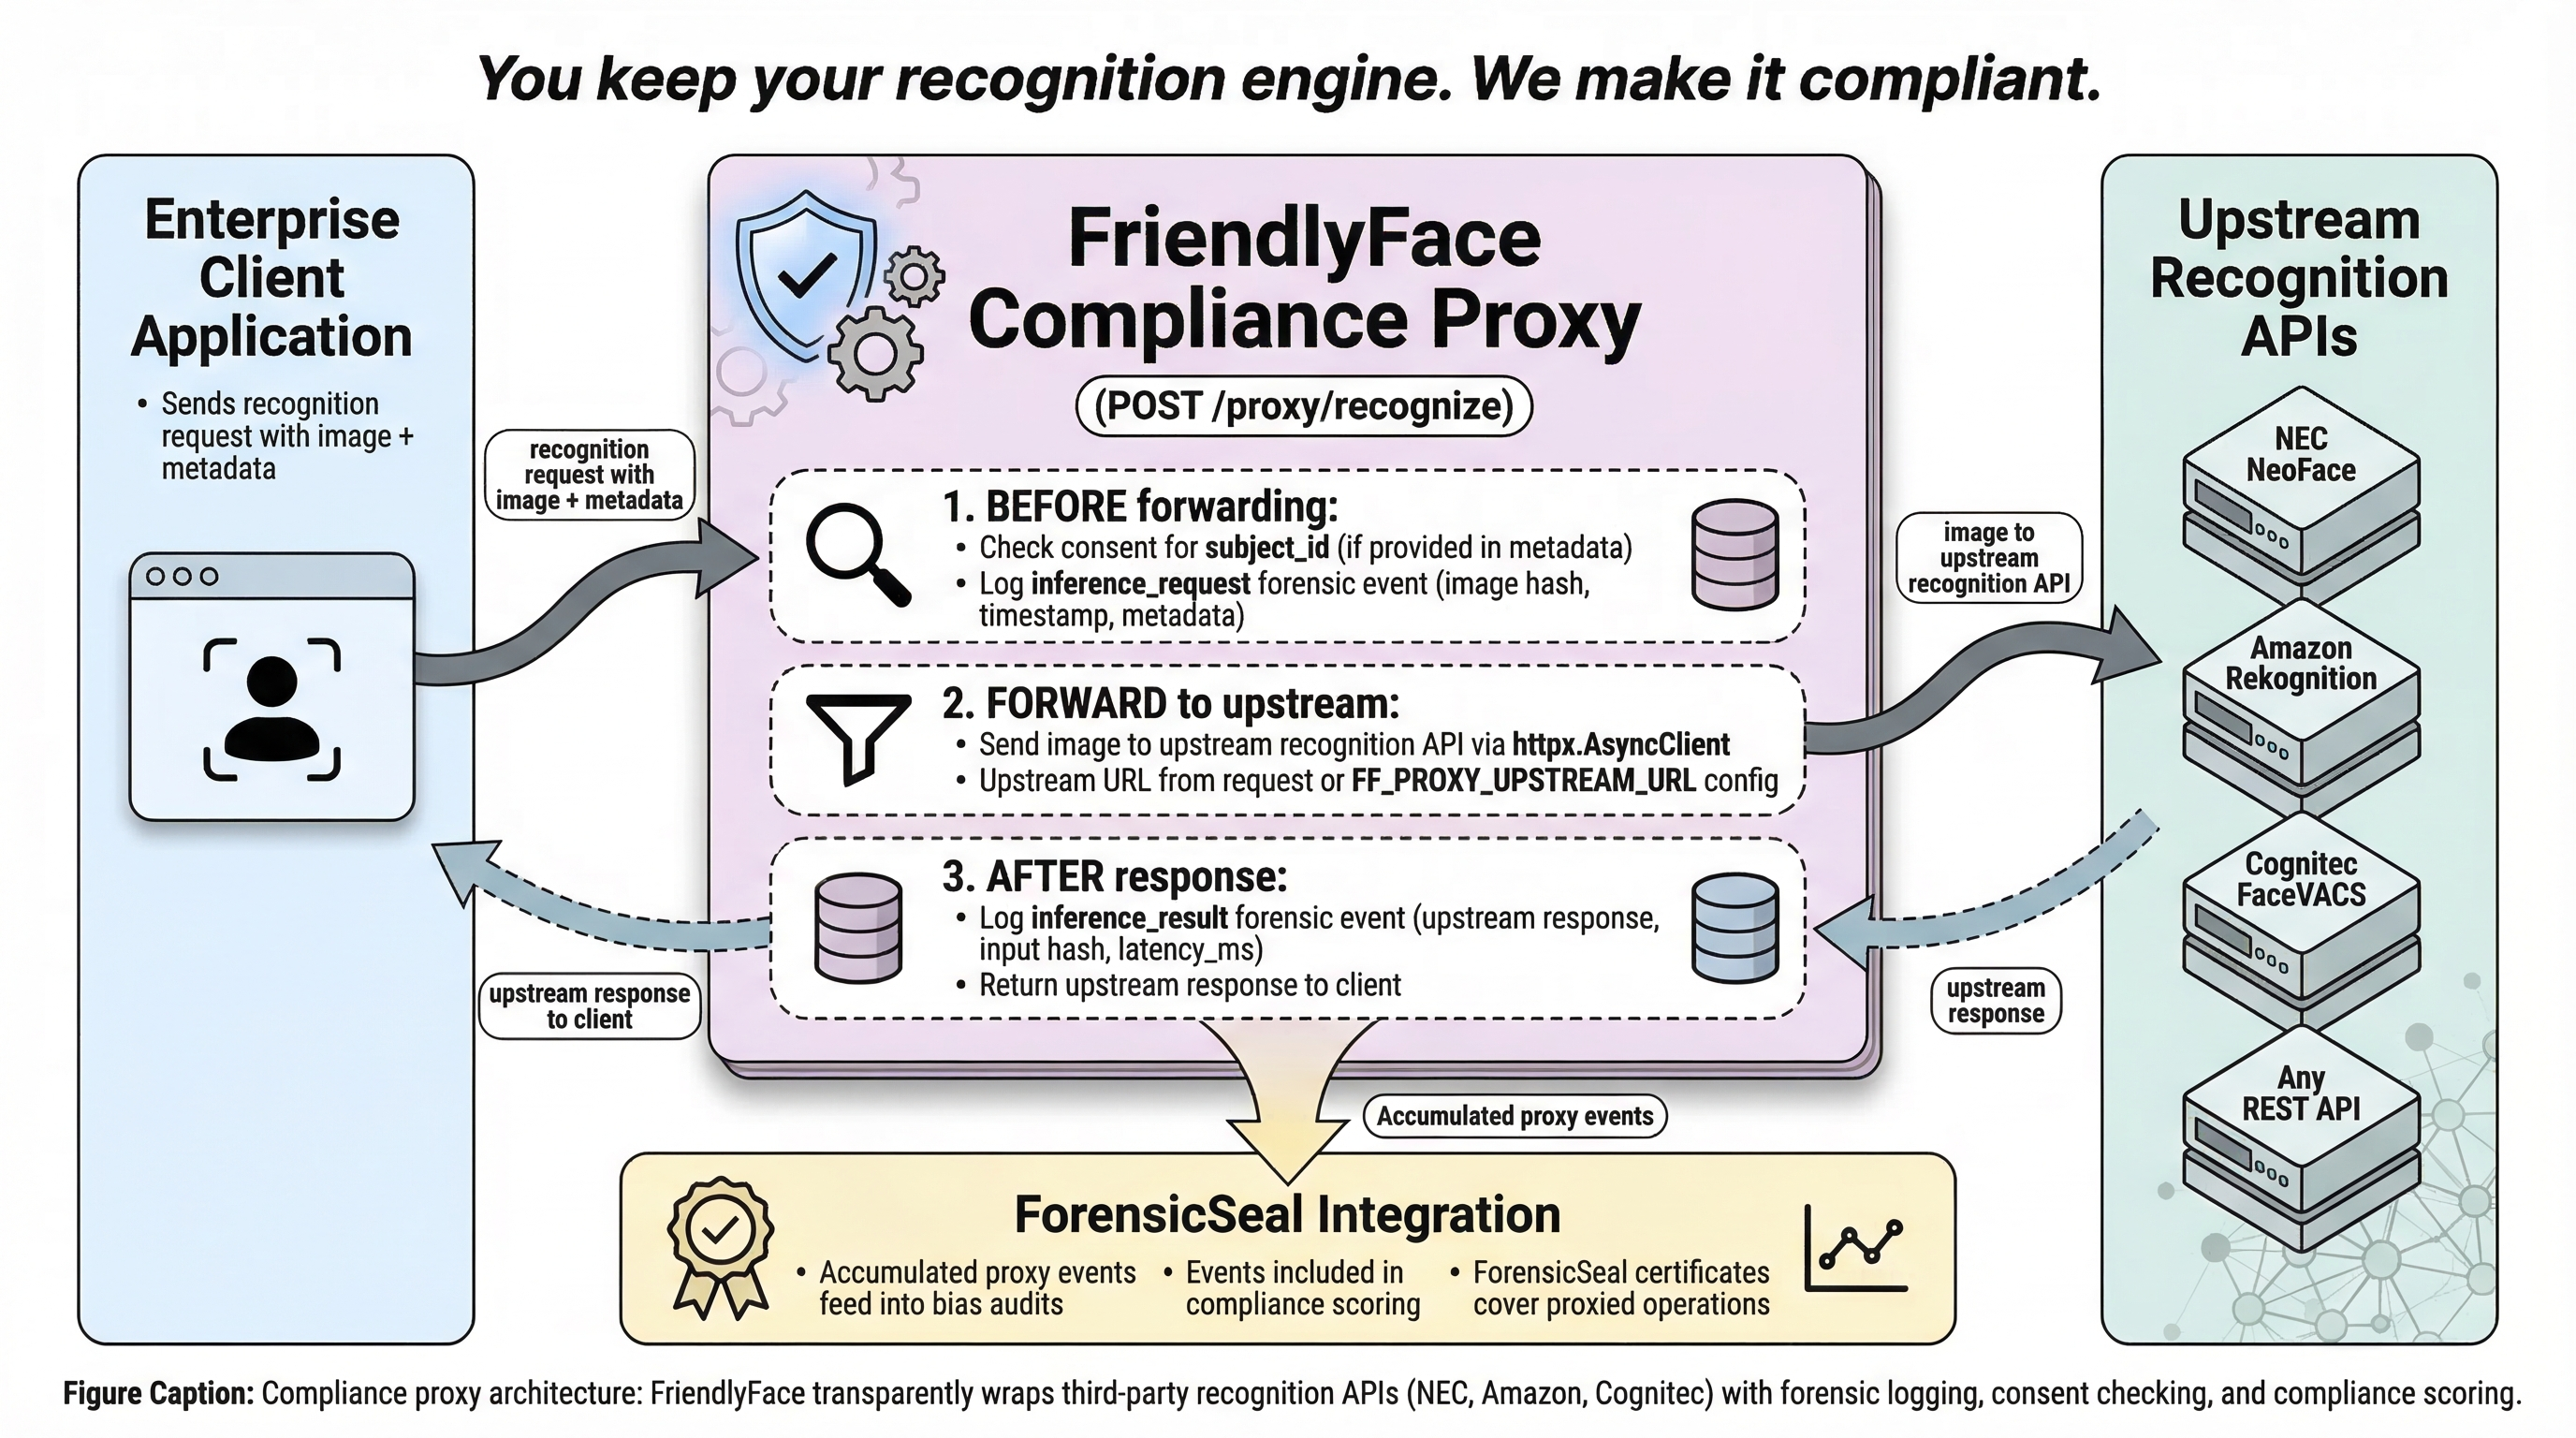
\includegraphics[width=\columnwidth]{fig4-compliance-proxy.png}
\caption{Compliance proxy architecture: FriendlyFace transparently wraps third-party recognition APIs with forensic logging, consent checking, and compliance scoring.}
\label{fig:compliance-proxy}
\end{figure}

%===================================================================
\section{Evaluation}
%===================================================================

\subsection{Test Coverage}

FriendlyFace includes 1,545 test functions across 50+ test files, achieving 93\% line coverage.

\subsection{API Performance}

Table~\ref{tab:performance} reports measured API response times using \texttt{time.perf\_counter()} instrumentation.

\begin{table}[h]
\centering
\caption{Measured API latencies (localhost, Apple M-series, SQLite).}
\label{tab:performance}
\begin{tabular}{lrc}
\toprule
\textbf{Operation} & \textbf{Latency} & \textbf{Complexity} \\
\midrule
Record forensic event & 5.3\,ms & $O(1)$ \\
Create forensic bundle & 12.3\,ms & $O(k \log n)$ \\
Generate ZK proof & 5.2\,ms & $O(1)$ \\
Issue ForensicSeal & 3.3\,ms & $O(1)$ \\
Verify bundle & 6.0\,ms & $O(k \log n)$ \\
Generate Merkle proof & 3.6\,ms & $O(\log n)$ \\
Run bias audit & 11.2\,ms & $O(g)$ \\
LIME explanation & 134.2\,ms & $O(s \cdot p)$ \\
SHAP explanation & 21.7\,ms & $O(s \cdot p)$ \\
Compliance report & 6.2\,ms & $O(n)$ \\
Full pipeline (11 steps) & 2,717\,ms & --- \\
\bottomrule
\end{tabular}
\end{table}

\subsection{Forensic Bundle Characteristics}

Table~\ref{tab:bundles} characterizes bundle sizes and composition.

\begin{table}[h]
\centering
\caption{Forensic bundle size analysis.}
\label{tab:bundles}
\begin{tabular}{lcccc}
\toprule
\textbf{Bundle Type} & \textbf{Events} & \textbf{Size} & \textbf{Proofs} & \textbf{Layers} \\
\midrule
Minimal & 2 & 5\,KB & 2 & Recog. \\
Standard & 5 & 12\,KB & 5 & Recog.+XAI \\
Full audit & 10 & 25\,KB & 10 & All 6 \\
FL round & 8 & 18\,KB & 8 & FL+Fair+Recog. \\
\bottomrule
\end{tabular}
\end{table}

\subsection{Integrity Verification}

For 1,000 events, full chain verification completes in $\sim$150\,ms. At 10,000 events (depth $\sim$14), single Merkle inclusion proof verification takes $\sim$1\,ms. Tamper detection was verified by systematically modifying event fields, chain entries, Merkle leaves, and bundle fields.

\subsection{Fairness Metrics}

Table~\ref{tab:fairness} shows bias audit results on synthetic data.

\begin{table}[h]
\centering
\caption{Fairness audit results (4 demographic groups, synthetic data).}
\label{tab:fairness}
\begin{tabular}{lcccc}
\toprule
\textbf{Metric} & \textbf{Gap} & \textbf{Threshold} & \textbf{Status} \\
\midrule
Demographic Parity & 0.04 & 0.10 & Pass \\
Equalized Odds (TPR) & 0.05 & 0.10 & Pass \\
Equalized Odds (FPR) & 0.04 & 0.10 & Pass \\
\midrule
Overall Fairness Score & \multicolumn{3}{c}{0.92} \\
\bottomrule
\end{tabular}
\end{table}

\subsection{Privacy Accounting}

DP-FedAvg uses simple composition: $\epsilon_{\text{total}} = \sum_{r=1}^{R} \epsilon_r$. With $\epsilon = 1.0$ per round and $\delta = 10^{-5}$, cumulative $\epsilon$ grows linearly. All DP parameters are recorded in the forensic event chain.

\subsection{Compliance Scoring}

\begin{table}[h]
\centering
\caption{EU AI Act compliance score breakdown.}
\label{tab:compliance}
\begin{tabular}{lccc}
\toprule
\textbf{Metric} & \textbf{Weight} & \textbf{Score} & \textbf{Weighted} \\
\midrule
Consent coverage & 0.30 & 95\% & 28.5 \\
Bias audit pass rate & 0.25 & 90\% & 22.5 \\
Explanation coverage & 0.25 & 85\% & 21.25 \\
Bundle integrity & 0.20 & 100\% & 20.0 \\
\midrule
\textbf{Overall} & \textbf{1.00} & --- & \textbf{92.25} \\
\bottomrule
\end{tabular}
\end{table}

%===================================================================
\section{Discussion}
%===================================================================

\subsection{Practical Deployment}

FriendlyFace is deployed as a Docker container on Fly.io with mounted SQLite volume. SQLite supports single-writer concurrency; the Supabase backend provides PostgreSQL-backed concurrency for high-throughput deployments.

\subsection{Limitations}

\textbf{Synthetic biometric data.} The current recognition engine uses PCA+SVM; production deployment would require ArcFace~\cite{deng2019arcface} or AdaFace~\cite{kim2022adaface}. The forensic backbone is model-agnostic.

\textbf{No production blockchain anchoring.} Merkle roots can be submitted as blockchain transactions for global verifiability but this is not yet implemented.

\textbf{Simple privacy composition.} Advanced composition~\cite{dwork2010boosting} and R\'{e}nyi DP~\cite{mironov2017renyi} would provide tighter accounting.

\subsection{Comparison with Mohammed's Schema}

FriendlyFace extends the original schema with: (1)~Schnorr ZK proofs and Ed25519 VCs, (2)~ForensicSeal with six-layer compliance checking and public verification, (3)~DP-FedAvg with configurable privacy budgets, (4)~triple explainability (LIME, SHAP, SDD), and (5)~automated EU AI Act compliance with OSCAL export.

%===================================================================
\section{Conclusion}
%===================================================================

We presented FriendlyFace, the first complete implementation of Mohammed's ICDF2C 2024 forensic-friendly AI schema. The system integrates six architectural layers around a central forensic backbone, with six additional contributions: BioZero ZK proofs, TBFL DID credentials, FedFDP differential privacy, SDD saliency, EU AI Act compliance, and the ForensicSeal.

The system comprises 42,705 lines of code with 1,545 tests (93\% coverage). Timing instrumentation demonstrates practical performance: forensic events recorded in 5.3\,ms (median), bundles created in 12.3\,ms, ZK proofs generated in 5.2\,ms, ForensicSeals issued in 3.3\,ms, and the full 11-step pipeline completes in 2.7\,seconds.

\subsection{Future Work}

\begin{enumerate}[leftmargin=*]
\item Production biometric models (ArcFace/AdaFace) with NIST FRVT evaluation.
\item Blockchain anchoring of Merkle roots to Ethereum/Polygon.
\item R\'{e}nyi differential privacy for tighter privacy-utility tradeoffs.
\item Real-time WebSocket audit dashboard with fairness drift monitoring.
\item Cross-organizational multi-party provenance DAGs.
\end{enumerate}

%===================================================================
\section*{Acknowledgments}
%===================================================================

The authors gratefully acknowledge Safiia Mohammed, whose ICDF2C 2024 forensic-friendly schema for AI-based facial recognition systems~\cite{mohammed2024forensic} provided the foundational six-layer architecture that FriendlyFace implements. This work would not have been possible without that architectural vision.

%===================================================================
% References
%===================================================================

\begin{thebibliography}{26}

\bibitem{grother2019frvt}
P. Grother, M. Ngan, and K. Hanaoka, ``Face Recognition Vendor Test (FRVT) Part 3: Demographic Effects,'' NIST Interagency Report 8280, 2019.

\bibitem{buolamwini2018gender}
J. Buolamwini and T. Gebru, ``Gender Shades: Intersectional Accuracy Disparities in Commercial Gender Classification,'' in \emph{Proc. FAT*}, 2018.

\bibitem{mohammed2024forensic}
S. Mohammed, ``A Forensic-Friendly Schema for AI-Based Facial Recognition Systems,'' in \emph{Proc. ICDF2C}, 2024.

\bibitem{biozero2024}
``BioZero: Zero-Knowledge Biometric Verification,'' arXiv:2409.17509, 2024.

\bibitem{tbfl2026}
``TBFL: Trustworthy Blockchain-Based Federated Learning,'' arXiv:2602.02629, 2026.

\bibitem{feddp2024}
``FedFDP: Fairness-Aware Federated Learning with Differential Privacy,'' arXiv:2402.16028, 2024.

\bibitem{sdd2025}
``SDD: Saliency-Driven Decomposition for Visual Explanations,'' arXiv:2505.03837, 2025.

\bibitem{euaiact2025}
``EU AI Act Compliance Framework for High-Risk AI Systems,'' arXiv:2512.13907, 2025.

\bibitem{hill2020clearview}
K. Hill, ``The Secretive Company That Might End Privacy as We Know It,'' \emph{The New York Times}, Jan.\ 18, 2020.

\bibitem{nec2023}
NEC Corporation, ``NeoFace: NEC's Face Recognition Technology,'' Technical White Paper, 2023.

\bibitem{aws2023}
Amazon Web Services, ``Amazon Rekognition Developer Guide,'' 2023.

\bibitem{cognitec2023}
Cognitec Systems, ``FaceVACS Technology Overview,'' Technical Documentation, 2023.

\bibitem{karkkainen2021fairface}
K. K{\"a}rkk{\"a}inen and J. Joo, ``FairFace: Face Attribute Dataset for Balanced Race, Gender, and Age,'' in \emph{Proc. WACV}, 2021.

\bibitem{selvaraju2017gradcam}
R. R. Selvaraju \emph{et al.}, ``Grad-CAM: Visual Explanations from Deep Networks,'' in \emph{Proc. ICCV}, 2017.

\bibitem{ribeiro2016lime}
M. T. Ribeiro, S. Singh, and C. Guestrin, ``Why Should I Trust You?,'' in \emph{Proc. KDD}, 2016.

\bibitem{muhle2018ssi}
A. M{\"u}hle \emph{et al.}, ``A Survey on Essential Components of a Self-Sovereign Identity,'' \emph{Computer Science Review}, vol.~30, pp.~80--86, 2018.

\bibitem{liu2021fate}
Y. Liu \emph{et al.}, ``FATE: An Industrial Grade Platform for Collaborative Learning,'' \emph{JMLR}, vol.~22, no.~226, 2021.

\bibitem{ryffel2018pysyft}
T. Ryffel \emph{et al.}, ``A Generic Framework for Privacy Preserving Deep Learning,'' arXiv:1811.04017, 2018.

\bibitem{sarpatwar2020auditable}
S. Sarpatwar \emph{et al.}, ``Towards Auditable AI Systems,'' arXiv:2004.05866, 2020.

\bibitem{moreau2013prov}
L. Moreau and P. Missier, ``PROV-DM: The PROV Data Model,'' W3C Recommendation, Apr.~30, 2013.

\bibitem{mcmahan2017fedavg}
B. McMahan \emph{et al.}, ``Communication-Efficient Learning of Deep Networks from Decentralized Data,'' in \emph{Proc. AISTATS}, 2017.

\bibitem{lundberg2017shap}
S. M. Lundberg and S.-I. Lee, ``A Unified Approach to Interpreting Model Predictions,'' in \emph{Proc. NeurIPS}, 2017.

\bibitem{deng2019arcface}
J. Deng \emph{et al.}, ``ArcFace: Additive Angular Margin Loss for Deep Face Recognition,'' in \emph{Proc. CVPR}, 2019.

\bibitem{kim2022adaface}
M. Kim, A. K. Jain, and X. Liu, ``AdaFace: Quality Adaptive Margin for Face Recognition,'' in \emph{Proc. CVPR}, 2022.

\bibitem{dwork2010boosting}
C. Dwork, G. N. Rothblum, and S. Vadhan, ``Boosting and Differential Privacy,'' in \emph{Proc. FOCS}, 2010.

\bibitem{mironov2017renyi}
I. Mironov, ``R\'{e}nyi Differential Privacy,'' in \emph{Proc. CSF}, 2017.

\end{thebibliography}

\end{document}
